\documentclass[11pt]{article}
\usepackage[utf8]{inputenc}
\usepackage[french]{babel}
\usepackage[T1]{fontenc}
\usepackage{verbatim}
\usepackage{graphicx}
\usepackage{amsmath}
\usepackage{eurosym}
\usepackage{textcomp}
\usepackage{graphicx}
\author{Contzen Laurent, Corvalan Gabriel}
\title{NaluRSS}
\date{14 Décembre 2009}

\begin{document}

\begin{titlepage}
\begin{flushleft}
Contzen Laurent \\
Corvalan Gabriel \\
\end{flushleft}
\begin{center}
\vspace{65mm}\LARGE{\textbf{INFO-H-303 - Bases de données} :\\
NaluRSS}
\end{center}
\begin{flushright}
\vspace{70mm}
Année Académique 2009-2010.
\end{flushright}
\end{titlepage}
\tableofcontents
\newpage

\section{Introduction}
Dans le cadre de ce projet du cours de bases de données nous avons du développer un agrégateur de flux rss. Un flux rss est un fichier xml\footnote{eXtensible Markup Language} contenant des informations sur les dernières mises à jour d'un site internet. Une fois ce flux intégré dans un agrégateur l'utilisateur est automatiquement tenu au courant de ces mises à jour. Le grand intérêt de ceci est de pouvoir avoir les nouvelles ionformations de tous nos sites préférés en une fois dans une seule même interface plutot que de devoir aller sur chaque site un à un.
\section{Présentation de NaluRSS}
NaluRSS est entièrement écrit en xhtml\footnote{eXtensible HyperText Markup Language}/css\footnote{Cascading Style Sheet} et php\footnote{PHP: HyperText Preprocessor} et enregistre les informations dans une base de données MySQL. Il a été pensé pour être le plus simple d'utilisation possible pour l'utilisateur. Ses principales fonctionnalités sont :
\begin{itemize}
\item{Un système multi-utilisateurs}
\item{La possibilité d'être \og ami \fg avec un autre utilisateur}
\item{La possibilité de partager une nouvelle d'un flux avec ses \og amis \fg, et ce avec un commentaire}
\item{La possibilité d'ajouter ou supprimer des \og amis \fg}
\item{L'ajout et la suppression de feeds}
\item{L'affichage des flux en version condensée (juste les titres des articles) ou en version complète (les titres et descriptions des articles)}
\item{L'affichage des flux des \og amis \fg (chaque élément partagé par une personne fait partie de son flux personnel)}*
\item{L'affichage d'un unique article avec sa description}
\item{La possibilité de s'inscrire sur le site}
\item{Et bien d'autres}
\end{itemize}
Voici une capture d'écran de la page d'accueil :
\begin{figure}[!ht]
\begin{center}
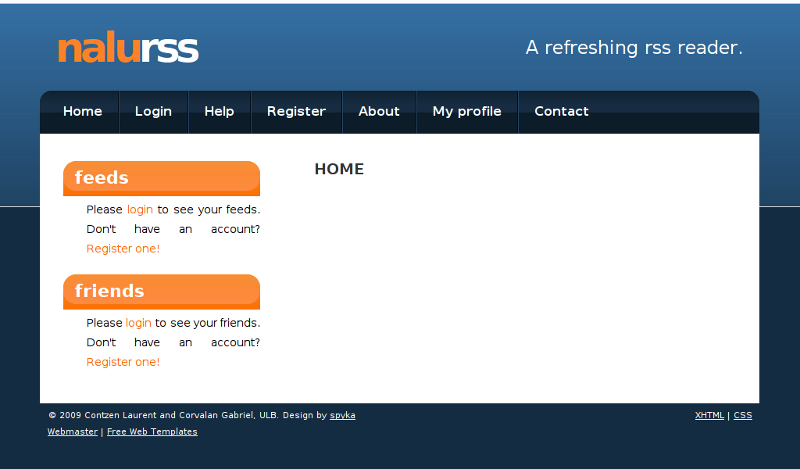
\includegraphics[width=14cm]{home.png}
\end{center}
\caption{Page d'accueil de NaluRSS pour un utilisateur non enregistré}
\label{home}
\end{figure}
\newline

\section{Script SQL DDL de création de la base de données}
\begin{verbatim}
SET SQL_MODE="NO_AUTO_VALUE_ON_ZERO";

CREATE DATABASE `db_projet` DEFAULT CHARACTER SET latin1 COLLATE latin1_swedish_ci;
USE `db_projet`;



DROP TABLE IF EXISTS `Comments`;
CREATE TABLE IF NOT EXISTS `Comments` (
  `Email` varchar(200) NOT NULL,
  `Text` text NOT NULL,
  `URLFeed` varchar(400) NOT NULL,
  `URLItem` varchar(400) NOT NULL,
  `Date` datetime NOT NULL,
  PRIMARY KEY (`Email`,`URLFeed`,`URLItem`)
) ENGINE=MyISAM DEFAULT CHARSET=latin1;



DROP TABLE IF EXISTS `FeedItems`;
CREATE TABLE IF NOT EXISTS `FeedItems` (
  `URLFeed` varchar(400) NOT NULL,
  `URLItem` varchar(400) NOT NULL,
  PRIMARY KEY (`URLFeed`,`URLItem`)
) ENGINE=MyISAM DEFAULT CHARSET=latin1;



DROP TABLE IF EXISTS `Feeds`;
CREATE TABLE IF NOT EXISTS `Feeds` (
  `URL` varchar(400) CHARACTER SET latin1 NOT NULL,
  `Name` varchar(200) CHARACTER SET latin1 NOT NULL,
  `Description` varchar(200) CHARACTER SET latin1 NOT NULL,
  `Link` varchar(400) CHARACTER SET latin1 NOT NULL,
  PRIMARY KEY (`URL`)
) ENGINE=MyISAM DEFAULT CHARSET=utf8 COLLATE=utf8_unicode_ci;



DROP TABLE IF EXISTS `Friends`;
CREATE TABLE IF NOT EXISTS `Friends` (
  `EmailA` varchar(200) NOT NULL,
  `EmailB` varchar(200) CHARACTER SET utf8 COLLATE utf8_unicode_ci NOT NULL,
  `Date` datetime NOT NULL,
  `Accepted` tinyint(1) NOT NULL,
  PRIMARY KEY (`EmailA`,`EmailB`)
) ENGINE=MyISAM DEFAULT CHARSET=latin1;



DROP TABLE IF EXISTS `Items`;
CREATE TABLE IF NOT EXISTS `Items` (
  `URL` varchar(400) NOT NULL,
  `Title` varchar(200) NOT NULL,
  `Date` datetime NOT NULL,
  `Description` text NOT NULL,
  PRIMARY KEY (`URL`)
) ENGINE=MyISAM DEFAULT CHARSET=latin1;



DROP TABLE IF EXISTS `Reads`;
CREATE TABLE IF NOT EXISTS `Reads` (
  `Email` varchar(200) NOT NULL,
  `URLItem` varchar(400) NOT NULL,
  `URLFeed` varchar(400) NOT NULL,
  `Date` datetime NOT NULL,
  PRIMARY KEY (`Email`,`URLItem`,`URLFeed`)
) ENGINE=MyISAM DEFAULT CHARSET=latin1;



DROP TABLE IF EXISTS `Shares`;
CREATE TABLE IF NOT EXISTS `Shares` (
  `URLFeed` varchar(400) NOT NULL,
  `URLItem` varchar(400) NOT NULL,
  `Email` varchar(200) NOT NULL,
  `Note` text NOT NULL,
  `Date` datetime NOT NULL,
  PRIMARY KEY (`URLFeed`,`URLItem`,`Email`)
) ENGINE=MyISAM DEFAULT CHARSET=latin1;



DROP TABLE IF EXISTS `Subscriptions`;
CREATE TABLE IF NOT EXISTS `Subscriptions` (
  `Email` varchar(200) NOT NULL,
  `URL` varchar(400) NOT NULL,
  `Date` datetime NOT NULL,
  PRIMARY KEY (`Email`,`URL`)
) ENGINE=MyISAM DEFAULT CHARSET=latin1;



DROP TABLE IF EXISTS `Users`;
CREATE TABLE IF NOT EXISTS `Users` (
  `Email` varchar(200) CHARACTER SET utf8 COLLATE utf8_unicode_ci NOT NULL,
  `Password` varchar(20) CHARACTER SET utf8 COLLATE utf8_unicode_ci NOT NULL,
  `Nickname` varchar(20) CHARACTER SET utf8 COLLATE utf8_unicode_ci NOT NULL,
  `City` varchar(20) CHARACTER SET utf8 COLLATE utf8_unicode_ci NOT NULL,
  `Country` varchar(20) CHARACTER SET utf8 COLLATE utf8_unicode_ci NOT NULL,
  `Avatar` text CHARACTER SET utf8 COLLATE utf8_unicode_ci NOT NULL,
  `Biography` varchar(50) CHARACTER SET utf8 COLLATE utf8_unicode_ci DEFAULT NULL,
  `SubscribeDate` datetime NOT NULL,
  `FeedURL` varchar(400) CHARACTER SET utf8 COLLATE utf8_unicode_ci NOT NULL,
  PRIMARY KEY (`Email`)
) ENGINE=MyISAM DEFAULT CHARSET=latin1;
\end{verbatim}
\section{Requêtes demandés en algèbre relationnel}
\subsection{R1}
\noindent $AcceptedFriends \longleftarrow \pi_{EmailA, EmailB}(\sigma_{Accepted = 1}(Friends))$ \\
$UsersMails \longleftarrow \pi_{Email}(Users)$ \\
$temp \longleftarrow AcceptedFriends \ast \alpha_{EmailB : EmailC}(AcceptedFriends) \ast \alpha_{EmailB : EmailD}(AcceptedFriends) $ \\
$temp2 \longleftarrow \alpha_{EmailA : Email}(\pi_{EmailA}(\sigma_{EmailB \neq EmailC \wedge EmailB \neq EmailD \wedge EmailC \neq EmailD}(temp))) $ \\
$Result \longleftarrow UsersMails - temp2 $
\subsection{R2}
\noindent $FeedsX \longleftarrow \pi_{Email = X}(Subscriptions) $ \\

\subsection{R3}
\noindent $FeedsX \longleftarrow \pi_{Email = X}(Subscriptions) $ \\
$SharesX \longleftarrow \pi_{Email}(\sigma_{Email = X}(Shares))$ \\
$FriendsX \longleftarrow \alpha_{EmailA : Email}(\pi_{EmailA}(\sigma_{EmailA = X \wedge Accepted = 1}(Friends))) \cup \alpha_{EmailB : Email} (\pi_{EmailB}(\sigma_{EmailB = X \wedge Accepted = 1}(Friends)))$ \\
$Result \longleftarrow FeedsX - FriendsX - SharesX$


\section{Requêtes demandés en calcul relationnel tuple}
\subsection{R1}
$\{ User.Email \mid Friend(f) \wedge (f.EmailA \vee f.EmailB) \wedge (\not\exists f1(Friend(f1)) \mid (EmailA = User.Email \vee EmailB = User.Email)) \vee ((\exists f1(Friend(f1)) \mid (EmailA = User.Email \vee EmailB = User.Email)) \wedge (\not\exists f2(Friend(f2)) \mid (EmailA = User.Email \vee EmailB = User.Email))) \vee ((\exists f1(Friend(f1)) \mid (EmailA = User.Email \vee EmailB = User.Email)) \wedge (\exists f2(Friend(f2)) \mid (EmailA = User.Email \vee EmailB = User.Email)) \wedge (\exists f3(Friend(f3)) \mid (EmailA = User.Email \vee EmailB = User.Email)))$

\section{Requêtes demandés en SQL}
\subsection{R1}
SELECT * FROM Users WHERE (SELECT COUNT(*) FROM Friends WHERE (EmailA = Email AND Accepted = 0) OR (EmailB = Email AND Accepted = 0)) < 3
\subsection{R3}
SELECT URL FROM Subscriptions WHERE Email NOT IN ( \\
SELECT Email FROM Users WHERE Email IN (SELECT EmailB FROM Friends WHERE EmailA = 'X' AND Accepted = 1) OR Email IN (SELECT EmailA FROM Friends WHERE EmailB = 'X' AND Accepted = 1)) \\
AND URL NOT IN (SELECT URLFeed FROM Shares WHERE Email = 'X')


\section{Instructions d'installation}
\subsection{Pré-requis}
Afin d'installer NaluRSS il faut disposer d'un serveur sur lequel tournent un serveur web\footnote{Apache par exemple}, une base de données MySQL et un interpréteur PHP. Tout ceci se trouve facilement sur la plupart des hébergeurs ou s'installe très facilement en tant que serveur LAMP\footnote{Linux Apache Mysql Php}, WAMP\footnote{Windows Apache Mysql Php} ou encore MAMP\footnote{Mac Apache Mysql Php}. Le programme phpMyAdmin peut aussi être installé pour faciliter les interactions manuelles avec la base de données.
\subsection{Installation}
Une fois que nous avons un serveur *AMP fonctionnel en marche l'installation est extrèmement simple : il suffit de 
\begin{itemize}
\item{Décompresser l'archive dans le répertoire fixé par la configuration du serveur Apache}
\item{Ajuster le fichier config.ini selon la configuration désirée}
\item{Importer la structure de données}
\end{itemize}

\section{Scénario de démonstration}

\section{Explications diverses}
Le fichier \verb|config.ini| qui contient nottament le mot de passe d'accès à la base de données est protégé par un fichier \verb|.htaccess| afin d'éviter les accès depuis l'extérieur.

\section{Conclusion}
Nous avons donc ici un agrégateur de flux rss parfaitement utilisable en production si les fonctionnalités présentes suffisent, et facilement extensible à souhait sinon.

\section{Rapport de la première partie corrigé}
\subsection{Diagramme entité-association}
\begin{itemize}
\item{La date d'inscription d'un utilisateur doit être strictement inférieure à celle de la publication d'un de ses articles ou d'un de ses commentaires, et également inférieure à la date d'un début d'amitié.
Un utilisateur ne peut s'inscrire à son propre flux.}
\item{Dans une relation d'amité, un utilisateur ne peut être ami avec lui même.}
\item{Seul le champ Biography peut être vide car il est optionnel.}
\item{Le flux User est composé d'un ensemble de partages}
\item{Un utilisateur ne peut commenter qu'une fois un Item}
\item{Un Item ne peut être défini qu'une fois comme lu par un User}
\item{Une Item peut appartenir à plusieurs flux}
\item{Un utilisateur ne peut partager un Item que s'il a souscrit aux flux duquel provient l'Item}
\end{itemize}
\begin{figure}[!ht]
\begin{center}
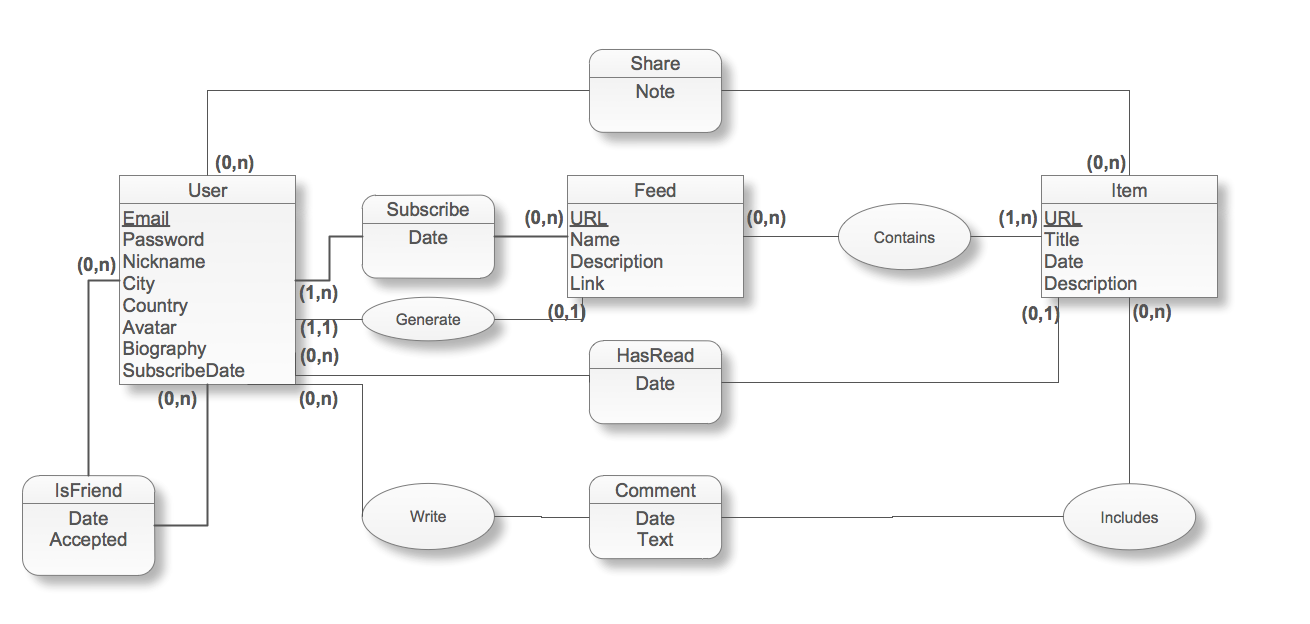
\includegraphics[width=14cm]{diagram.png}
\end{center}
\caption{Diagramme entité-association}
\label{giagram}
\end{figure}
\subsection{Traduction relationnelle}
\noindent \textbf{User} (\underline{Email}, Nickname, Country, City, Avatar, Subscription date, Biography, Password, URL) \\
 \newline
\textbf{IsFriend} (\underline{EmailA, EmailB}, Date, Accepted) \\
	IsFriend.EmailA référence User.Email \\
	IsFriend.EmailB référence User.Email \\
\newline
\textbf{Feed} (\underline{URL}, Name, Description, Link) \\
\newline
\textbf{Subscribe} (\underline{Email, URL}, Date) \\
	Subscribe.Email référence User.Email \\
	Subscribe.URL référence Feed.URL \\
\newline
\textbf{Item} (\underline{URL}, Title, Link, Date, Description) \\
\newline
\textbf{Contains} (\underline{URLfeed, URLitem}) \\
	Contains.URLfeed référence Feed.URL \\
	Contains.URLitem référence Item.URL \\
\newline
\textbf{HasRead} (\underline{Email, URLfeed, URLitem}, Date) \\
	HasRead.Email référence User.Email \\
	HasRead.URLfeed référence Feed.URL \\
	HasRead.URLitem référence Item.URL \\
\newline
\textbf{Comment} (\underline{EmailWriter, URLfeed, URLitem}, Text, Date) \\
	Comment.EmailWriter référence User.Email \\
	Comment.URLfeed référence Feed.URL \\
	Comment.URLitem référence Item.URL \\
\begin{itemize}
\item{IsFriend.EmailA != IsFriend.EmailB}
\item{User.SubscriptionDate <= IsFriend.Date}
\item{User.SubscriptionDate <= Subscribe.Date}
\item{User.SubscriptionDate <= HasRead.Date}
\item{User.SubscriptionDate <= Comment.Date}
\item{User.Biography peut être vide}
\end{itemize}
\subsection{Hypothèses et justifications}
Nous considérons ici qu'un flux généré par un utilisateur n'est pas différent d'un autre flux, la seul exception sera l'URL, en effet ici l'url ne pourra pas ressembler à une URL http (http://...), nous pourrons définir un type de schéma URL propre à notre implémentation. Par exemple rss://User.Email. Sinon pour le reste, nous restons proche des spécification RSS, bien que nous ne tiendrons pas compte d'une série de champ optionnel pour des soucis de simplification.

\end{document}
